%!TEX root = ../template.tex
\chapter{Background}\label{cha:background}

\section{Systems Programming Languages}\label{sec:systems-programming}

The definition of the term \emph{systems programming language} is not agreed upon,
being somewhat flexible and ever-changing due to constant shift in requirements for applications.

Before the cloud, in the age of C, a systems programming language would
most likely be a language able to provide an adequate interface between the programmer and the machine.
Nowadays, the definition is more vague, as machines and software grow in complexity,
and the definition of system grows from single computer to a distributed system,
interfacing with the hardware in a more direct fashion is mostly not required.
Systems programming languages become about being able to produce a standalone
binary able to run on a variety of machines without requiring extra software.

\subsection{C}

C is a general-purpose programming language, while it can be considered a high-level programming language
when put besides assembly, it also fits the description of a low-level level programming language when besides languages like Python.
It was originally designed by Dennis Ritchie for the PDP-11 and has been around since 1972 \autocite{Kernighan1988},
C is by no means modern, being older than myself and most likely to outlive me.

Designed in a different time, C's mental model is also different, the language is simple and straight forward,
the designers had goals to achieve and designed the language with them in mind.
Such mentality is noticeable when using the language,
it is simple as the hardware was and the level of control C provides is unparalleled,
being both a major benefit and a hindrance.
An expert programmer is able to take advantage of the language to produce highly-efficient software,
but a novice programmer will often find himself battling memory and pointer management bugs.

The language influence echoes in the modern languages,
whether in the form of syntax (i.e. the famous C-style syntax) or in the problems it tries to solve.
Languages such as Java take from C their syntax as well as one problem to solve, memory management;
other languages like Julia \autocite{Bezanson2017} aim to achieve similar performance.

While not as popular as other languages, C was able to stay relevant in the modern development landscape,
some of the most used software in the world is either written or powered by C.
The Linux kernel, which powers servers, the world's most powerful computers
and serves as a base for Android and other mobile devices,
git, Redis and nginx are also software examples which reached the top of their respective fields.

\subsection{C++}

Introduced in 1985 as an extension to C; the author, Bjarne Stroustrup writes:

\begin{displayquote}[{\autocite[Section 1.2]{Stroustrup1986}}]
    C++  is  based  on  the idea of providing both:
    \begin{compactitem}
        \item direct mappings of built-in operations and types to hardware to provide efficient memory use and efficient low-level operations, and
        \item affordable and flexible abstraction mechanisms to provide user-defined types with the same notational support, range of uses, and performance as built-in types.
    \end{compactitem}
\end{displayquote}

The language has since gone on to conquer the programming world, being used in a wide variety of software and hardware.
Currently, companies such as Google, Amazon and Microsoft have widespread adoption of C++ in their codebases.
Industries requiring the best performance as possible of the host, such as scientific computing,
financial software, AAA games and visual effects will most likely be running C++.

Just like C, C++ is far from perfect.
The language is enormous, with very complicated parts (e.g. templates) and compilation for big projects is very slow,
the author acknowledges this in \autocite{Torre2014}.
Furthermore, as the language provides a high level of control over the system, it has manual memory management,
suffering from the same problems as C.
Even with smart pointers (e.g. \texttt{unique\_ptr}) the problem is not considered solved,
as they introduce overhead in the most demanding applications.


\subsection{Ada}

Ada was developed in 1980, during a standardization effort in the USA's Department of Defense,
with the goal of unifying projects spanning over 450 programming languages \autocite{Ada2021}.
Ada's main focus was the development of embedded applications,
currently the Ada language is mostly used in the critical domain due to the strong emphasis on safety,
some Ada success stories are the London Metro Victoria Line and the Paris Metro Line \autocite{SIGAda2021}.
The language is also used in several other domains, such as aviation, space vehicles, financial systems and more \autocite{Feldman2014}.

In comparison with the other languages in this section, Ada is eclipsed, barely showing in the GitHub rankings \autocite{Palmer2021}.
However, given that Ada's compiler is mostly a product, it makes sense that most Ada code is not open-source.
Regardless, when one views the list of features Ada has, the first arising question is “\emph{why is Ada not popular?}”.

An old article in AdaPower \autocite{Heaney1998} provides some possible insight over the question,
referring to the compiler's price and the Hoare's harsh critics.
From my point of view, the critics to the compiler and ecosystem pricing still make sense,
as access to the full tooling is limited.
The lack of programmers goes on to deepen the lack of adoption in the industry
and this cycle ends up limiting Ada's reach in the market.

\subsection{Go}

The Go programming language (or \texttt{golang}) is a Google project,
according the language folklore, it was designed by the authors while they waited for their C++ code to compile.
Go tried to address several of the criticisms to C, namely memory management,
which it solved by using a garbage collector.
While it has made a name for itself in the network and distributed systems sector,
being the main language behind projects like Docker \autocite{Docker2021} and Kubernetes \autocite{Kubernetes2021},
Go's categorization as a systems programming language can be discussed.

Sometimes, however, the performance might not be enough,
as was the case for Discord, the popular internet voice server company, as demand increased,
Go was not able to meet the expected performance requirements and the company replaced it with Rust \autocite{Howarth2020}.
In \autocite{Torre2014}, one of Go's authors, Rob Pike, says that he regrets categorizing Go as a systems programming language,
being rather a server programming language that evolved into a cloud infrastructure language.
Regardless of discussion, Go has proven to be a viable alternative to existing counterparts,
compromising extreme performance in name of safety and simplicity.

\subsection{Summary}

I reviewed four system programming languages, suited for different kinds of environments,
C, C++ and Ada can be considered the traditional system languages kind, with a strong emphasis on efficiency
and support for embedded devices.
Go on the other hand, could be considered a new generation systems programming language, a language for cloud infrastructure.
Among the four, only Ada places strong emphasis on safety, with several features allowing for more guarantees at compile time,
such as contract based programming and non-nullable types by default,
being the only one which does not suffer from the “\emph{billion dollar mistake}” \autocite{Hoare2009}.

\section{The Rust Language}\label{sec:rust-lang}

Rust is a fairly recent systems programming language,
it started as a side project of the author Graydon Hoare and the language public history dates back to 2010 \autocite{Hoare2010}.
In 2012 Mozilla picked up Rust to help develop the Servo browser engine, the successor to the previous Gecko engine;
as a way to test Rust's capabilities \autocite{Klabnik2016}.

\subsection{What makes Rust different?}

In comparison with other languages, one of the first things someone new to Rust ought to notice is the emphasis put on safety.
Being a competitor to C++ and achieving memory safety while still providing C++-level performance is quite an accomplishment.
Rust, however, also aims to allow users to be productive without sacrificing safety or performance.

The key to all the promises Rust makes is the ownership system and borrow checker.
The borrow checker is a completely new mechanism when compared with other mainstream languages.
However, it is a product of years of research both in academia and the industry.
This mechanism merits most of Rust's accomplishments and also the biggest problem, the learning curve.
While Rust has become more accessible over the years,
ownership and the borrow checker still require some effort on the part of the developer to learn.
I provide a small overview of ownership, the borrow checker and their part in Rust's promise of “\emph{fearless concurrency}”.


\subsection{Ownership}\label{sec:rust-lang:ownership}

Ownership is the mechanism used by Rust to ensure no memory block stays allocated longer than it is required to.
Through ownership, the compiler is able to free memory when required,
inserting the respective deallocation calls in the output program.
Behind ownership, there are three rules:

\begin{displayquote}[{\autocite[Section 4.1]{RustBook2021}}]
    \begin{compactitem}
        \item Each value in Rust has a variable that’s called the owner.
        \item There can only be one owner at a time.
        \item When the owner goes out of scope, the value will be dropped.
    \end{compactitem}
\end{displayquote}

To illustrate the rules, consider \autoref{lst:rust-move}, where we have two variables \texttt{x} and \texttt{y}.
First, \texttt{"Hello"}\footnotemark~is assigned to \texttt{x}, thus \texttt{x} now owns \texttt{"Hello"}.
After, \texttt{x} is assigned to \texttt{y}, consider the second rule of ownership, since we can only have one owner,
\texttt{x}'s value ownership is transferred to \texttt{y}.
Since we transferred \texttt{x}'s value to \texttt{y}, \texttt{x} is no longer valid, consequently,
when compiling the code an error will be issued due to \texttt{x} being moved.

Notice how \texttt{String::from} is used instead of another type,
since \keyword{String} type does not implement \keyword{Copy} it can only be moved.
If the used type implemented \keyword{Copy}, the value would have been copied instead of moved.

\begin{listing}
    \begin{minted}{Rust}
let x = String::from("Hello");  // ok: `x` is assigned "Hello"
let y = x;                      // ok: `x` is moved into `y`
println!("{}", x);              // error: `x` was moved in the previous line
    \end{minted}
    \caption{Example of the move-by-default mechanism to enforce ownership.}
    \label{lst:rust-move}
\end{listing}

So far this illustrates the first two rules. The last rule can be considered invisible,
as it happens during compilation and the user would not notice it usually.
What happens is that at the end of the scope, any variable whose owner is in scope, will be freed.
While the developer is not required to explicitly free the memory, the compiler will insert the calls for the developer.

\subsection{Borrowing}\label{sec:rust-lang:borrowing}

If the developer could only copy or move memory the usability of the language would be severely limited.
For example, functions that read a variable and produce a new value,
not requiring the variable to be consumed would be impossible.
To cope with this, Rust allows values to be \emph{borrowed}, in other words,
the owner of the variable allows for it to be read by others.

To borrow a value, one writes \texttt{\&value}, this creates a read-only reference to \texttt{value}.
There can be an unlimited number of read-only references to a value, but only a single mutable reference.
This is discussed in \autoref{sec:rust-lang:concurrency}. Consider the example \autoref{lst:rust-borrow}.
In the example, \texttt{x} is now possible to be printed since it was not moved into \texttt{y}.
Rather, \texttt{y} borrowed \texttt{x} through a reference.

Going back to the rules (\autoref{sec:rust-lang:ownership}), Rust's references obey them just like all other values.
The variable containing them has ownership \emph{over the reference}; it still is a single owner
(if \mintinline{Rust}{let z = y;} was to be added, the reference would be copied instead of moved);
and finally, when the owner goes out of scope \emph{the reference is dropped}, but not the original value.

\begin{listing}
    \begin{minted}{Rust}
let x = String::from("Hello");  // ok: `x` is assigned "Hello"
let y = &x;                     // ok: `x` is borrowed to `y`
println!("{}", x);              // ok: `x` can be printed since it is still valid
    \end{minted}
    \caption{Example using borrowing to allow for more than one reader on the same variable.}
    \label{lst:rust-borrow}
\end{listing}

\subsubsection*{Mutable Borrows}

One last thing to consider are mutable borrows.
As previously discussed, in Rust it is possible to create multiple immutable references but only one mutable reference.
Regarding mutable references there are two cases to consider:

\paragraph{$N$ mutable references,} see \autoref{lst:rust-borrow-n-mut}.
Understanding why only one mutable reference can exist at a time is trivial,
as multiple mutable references to the same object would allow it to be mutated concurrently,
which could lead to inconsistent values.

\paragraph{$N$ immutable references and $1$ mutable reference,} see \autoref{lst:rust-borrow-n-immut-1-mut}.
The reason behind not allowing a mutable reference to coexist is similar.
Consider that each value can be executed by a different thread,
the first two (\texttt{r1} and \texttt{r2}) are only read and the third (\texttt{r3}) can be read and written.
While there will be no conflicts between writers, it is possible for the readers to read an inconsistent value,
since it can happen during the write operation.

\begin{listing}
    \begin{minted}{Rust}
let mut s = String::from("hello");
let r1 = &mut s; // ok: first mutable borrow
let r2 = &mut s; // error: `s` was mutably borrowed in the previous line
    \end{minted}
    \caption{Example error while using multiple mutable borrows over the same variable.}
    \label{lst:rust-borrow-n-mut}
\end{listing}

\begin{listing}
    \begin{minted}{Rust}
let mut s = String::from("hello");
let r1 = &s;     // ok: first immutable borrow
let r2 = &s;     // ok: second immutable borrow
let r3 = &mut s; // error: `s` was immutably borrowed in the previous lines
    \end{minted}
    \caption{Example error while using a mutable borrow in conjunction with immutable ones.}
    \label{lst:rust-borrow-n-immut-1-mut}
\end{listing}

\subsection{Concurrency}\label{sec:rust-lang:concurrency}

\begin{displayquote}[{\autocite[Section 16]{RustBook2021}}]
    Initially, the Rust team thought that ensuring memory safety and preventing concurrency problems were two separate challenges to be solved with different methods.
    Over time, the team discovered that the ownership and type systems are a powerful set of tools to help manage memory safety and concurrency problems!
    By leveraging ownership and type checking, many concurrency errors are compile-time errors in Rust rather than runtime errors.
\end{displayquote}

Rust provides several kinds of mechanisms to prevent concurrency related problems.
Mechanisms as \emph{message-passing}, \emph{shared-state} and
traits to enable developers to extend upon the existing abstractions.

\subsubsection*{Message-passing}

Rust's message-passing library is inspired on Go's approach to concurrency,
prioritizing message passing over other kinds of concurrent approaches, such as locking.

\begin{displayquote}[{\autocite[Concurrency]{Go2021}}]
    Do not communicate by sharing memory; instead, share memory by communicating.
\end{displayquote}

Rust defines channels which have two ends, the transmitter and the receiver.
The former can also be seen as the sender, and when is declared with the message type,
the latter is also declared with the message type, they can be the same or distinct.

The ownership system comes in when the transmitter sends a message,
when received the ownership of the message is taken on by the receiver end.
This enforces that values cannot be in both sides of the communication at the same time,
preventing concurrent accesses.

\subsubsection*{Shared-state}

Along with message-passing, Rust allows memory to be shared in a concurrent, safe way.
Just as before, Rust's ownership system also helps with mutexes' biggest problem, locking and unlocking.

In a language like Java, whenever a thread is able to call \texttt{lock} on a mutex,
it is required to call \texttt{unlock} on it, only then can other threads can use it.
The problem is that this approach is subject to human error,
forgetting to call unlock or calling unlock in the wrong place is possible.
Making use of the ownership system, Rust is able to know when the lock reached the end of the scope and should be dropped.

\subsection{Why Rust instead of Language X?}

The main obstacle between typestates and programming languages is the requirement for aliasing control.
In short, typestates are incompatible with aliasing (details are provided in \autoref{sec:typestates}).

So to implement a language from the ground up, it is required that aliasing is handled,
however, instead of building a new one, the goal is to extend an existing one, Rust.
As discussed in \autoref{sec:rust-lang:borrowing}, Rust's ownership system allows for aliasing control.
Using moves to enforce the consumption of values,
immutable references for pure functions and mutable ones for limited mutability,
it is possible to emulate typestates. This takes care of aliasing concerns.

When designing on top of another language, two more ingredients are required,
a powerful extension mechanism (i.e. Rust's macros, discussed in \autoref{sec:rust-macros})
and a strong type system, able to provide the necessary abstractions.
Rust provides both, the type systems goes as far as allowing zero-sized types,
allowing type-level abstractions to incur no runtime overhead.
This is a key ingredient in our DSL, aiming to provide the minimal possible runtime with an expressive language.

\section{Behavioral Types}\label{sec:behavioral-types}

As previously discussed, with the growth in software complexity, developers are required to develop better tools to tame such complexity.
Such tools require a theoretical body of work to support them, behavioral types are part of such body of work.
The theory behind them encompasses several domains, and they can be applied over a wide range of entities, from an object to a web service.

The work on behavioral types arose in the context of type systems able to capture properties of computations \autocite{Huttel2016}.
Session types and typestates are part of this field of study,
both capturing distinct property kinds while aiming for a common goal,
stronger type systems and better static assurances.

\begin{displayquote}[\autocite{Ancona2016}]
    Roughly speaking, a behavioral type describes a software entity, such as an object, a communication channel,
    or a Web Service, in terms of the sequences of operations that allow for a correct interaction among the involved entities.
\end{displayquote}

Behavioral types allow developers to model a protocol,
define the communication messages and possible interactions and
check that certain requirements are met when implementing.
Consider the protocol from \autoref{fig:login-protocol},
where a user tries to authenticate.
A developer can use it as a specification
(for simplicity consider the uppercase messages to be simple strings),
using behavioral types the developer could be able to specify the described interactions and all boilerplate could be generated for him.
While using strings as a payload is not very “\emph{interesting}”,
consider instead that the object in transit is an encrypted payload,
the boilerplate will take care of decryption and deserialization.
Furthermore, consider the constraint that \emph{all interactions end with a message from the server}.
If the specification has an interaction that is not compliant with such rule,
the code should not compile, raising an error.

\begin{figure}
    \centering
    \begin{tikzpicture}
        \tikzstyle{entity}=[rectangle, rounded corners, thick, draw=black, minimum width=15mm, minimum height=7mm]
        \tikzstyle{timeline}=[-Square, thick]
        \tikzstyle{message}=[->, thick]
        \node[entity] (client) at (0, 1) {Client};
        \node[entity] (server) at (0, -1) {Server};

        \draw[message] (1.5, 1) -- node[rotate=90, above] {\small{\texttt{LOGIN}}} ++(0, -2);
        \draw[message] (2.5, 1) -- node[rotate=90, above] {\small{username}} node[rotate=90, below] {\small{\keyword{String}}} ++(0, -2);
        \draw[message] (3.75, 1) -- node[rotate=90, above] {\small{password}} node[rotate=90, below] {\small{\keyword{String}}} ++(0, -2);

        \draw[message] (5.25, -1) -- node[rotate=90, above] {\small{\texttt{ACCEPTED}}} ++ (0, 2);

        \draw[message] (6.5, -1) -- node[rotate=90, above] {\small{\texttt{REJECTED}}} ++ (0, 2);

        \draw[thick] (client) to ++(5.5, 0);
        \draw[thick] (server) to ++(5.5, 0);

        \draw[timeline] (6, -1) to ++(1.5, 0);
        \draw[timeline] (6, 1) to ++(1.5, 0);

        \draw[dashed, semithick] (4.5, -1.25) rectangle (7, 1.25);
        \path (4.5, 1.25) -- node[above] {\emph{Choice}} (7, 1.25);
    \end{tikzpicture}
    \caption{
        Communication protocol example. The communication establishment step is omitted for simplicity.
        In this protocol the client tries to login to a service by sending a message
        \texttt{LOGIN} followed by the username and password, both of type \keyword{String}.
        The server then replies with either an \texttt{ACCEPTED} or \texttt{REJECTED}, if the login was successful or not, respectively.
    }
    \label{fig:login-protocol}
\end{figure}

\subsection{Session Types}

Session types are a subset of behavioral types, focused on communication,
from entities in a distributed system to threads in a computer.
Session types are based on process calculi and can be thought as “\emph{types for protocols}” \autocite{Honda1993, Honda1998}.
They elevate communication to the type level, allowing expressing them as types in a program,
in turn this enables the compiler to reason about the protocol during compile-time \autocite{Vasconcelos2006, Gay2015}.

In Rust, a channel is created with \mintinline{Rust}{let (tx, rx) = channel::<SenderT, ReceiverT>()},
where \texttt{SenderT} and \texttt{ReceiverT} are the types sent and received by the channel.
Channels are well-typed, meaning that if \mintinline{Rust}{SenderT = String},
sending another type over the channel will result in a type error.

% \begin{listing}
    \centering
    \begin{minted}{Rust}
enum Request {
    Login(String, String),       // login with: {username, password}
    SendMessage(String, String), // send message to a user: {user, message}
    CheckStatus(String),         // check the status of a given user: {user}
}
enum Reply {
    AuthOk,             // successful login
    AuthErr,            // failed login
    MessageOk,          // successful message
    UserStatus(String), // user status
}
fn communicate() {
    let (tx, rx) = channel<Request, Reply>();
    tx.send(Request::Login("foo", "bar"));
    match tx.recv() {
        // ...
    }
}
    \end{minted}
    \caption{
        Application login example, modelled using Rust's \keyword{enum}s
        (some channel details were omitted for simplicity).
        Reusing channels requires the developer to clump all states in a single \keyword{enum}.
        Better state management requires the use of more channels, neither approaches are ideal.
    }
    \label{lst:rust-login-chan}
\end{listing}

Session types extend on this notion, not only allowing for a single type to be sent or received,
but also model the protocol.
Consider \autoref{lst:rust-login-chan}, the example has unnecessary complexity,
for each receive the developer is required to match all possible replies.
Ideally, we declare the steps and possible outcomes beforehand.

For example, in plain English:
\begin{compactenum}
    \item Send login credentials.
    \item If successful, send a message to user \texttt{jmgd}.
    \item Otherwise, exit.
\end{compactenum}

And now using session types (\autoref{eq:session-types}
with syntax adapted from \autocite{Vasconcelos2006},
where the first four assignments ($:=$) are simple aliases, to simplify reading):

% \begin{figure}
    \begin{align*}
        \mathbf{Login}   & := \{user: \keyword{String},~password: \keyword{String}\}                                                                                                 \\
        \mathbf{Message} & := \{user: \keyword{String},~message: \keyword{String}\}                                                                                                  \\
        \mathbf{Status}  & := \{user: \keyword{String}\}                                                                                                                             \\
        \mathbf{SReply}  & := \{status: \keyword{String}\}                                                                                                                           \\
        Server           & = ~?\mathbf{Login}.\oplus\langle !Ok.?\mathbf{Message}.\oplus\langle Ok.End, Err.End \rangle, !Err.End\rangle                                             \\
        Client           & = ~!\mathbf{Login}.\&\langle ?Ok.\&\langle ?\mathbf{Status}.!\mathbf{SReply}, !\mathbf{Message}.\&\langle Ok.End, Err.End \rangle\rangle, ?Err.End\rangle
    \end{align*}
    \caption{Session type example, equivalent to \autoref{lst:rust-login-chan}.}
    \label{eq:session-types}
\end{figure}

Consider $!$ to be \emph{sends}, $?$ to be \emph{receives}, $.$ the \emph{sequence} operator finally,
$\&$ the \emph{choice offering} and $\oplus$ the \emph{choice selection}.
Using session types effectively offloads complexity to the type system,
resulting in more complex types, but simpler implementations,
since protocol compliance can be checked during compilation and boilerplate can be added by the compiler.
No message is matching required, the compiler does it for the developer.
Using session types it is possible to write it in a simpler form, where a type is assigned to each endpoint.
Notice how the server provides more than one operation, but the user does not call them all.

\subsection{Typestates}\label{sec:typestates}

\begin{displayquote}[{\autocite{Strom1983}}]
    ... traditional strong type checking was enhanced with \textbf{typestate checking}
    a new mechanism in which the compiler guarantees that for all execution paths,
    the sequence of operations on each variable obeys a finite state grammar associated with that variable's type.
\end{displayquote}

The first language to make use of typestates was NIL~\autocite{Strom1983},
afterwards languages like Hermes~\autocite{Strom1990} and Plaid~\autocite{Aldrich2009}
extended the concept with new techniques.

\subsubsection*{Automata}

A possible question on the reader's mind is “\emph{how are automata and typestates related?}”.
This section tries to address that question and exemplify how automata helps prove typestates properties.
It is possible to express typestates as automata, as the reader can observe in \autoref{fig:file-automata}.
Each state is a possible state the object can be in, transitions are done through methods.
Methods can either mutate the object state, such as \texttt{open} and \texttt{close},
or leave it unchanged, such as \texttt{nextLine}.

\begin{figure}
    \centering
    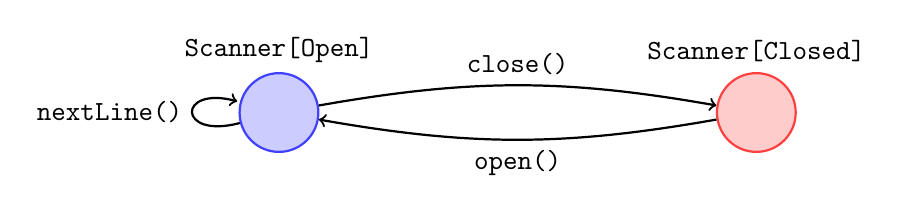
\begin{tikzpicture}
        \tikzstyle{open-file}=[circle, thick, draw=blue!75, fill=blue!20, minimum size=10mm]
        \tikzstyle{closed-file}=[circle, thick, draw=red!75, fill=red!20, minimum size=10mm]
        \tikzstyle{transition} = [->, thick];

        % \draw (0, 0) grid (\textwidth, 2);
        \node[open-file, label=above:\texttt{Scanner[Open]}] (open-file) at (0.25\textwidth, 1) {};
        \node[closed-file, label=above:\texttt{Scanner[Closed]}] (closed-file) at (0.75\textwidth, 1) {};
        \draw[transition]
        (open-file)
        edge[out=10, in=170] node[above] {\texttt{close()}}
        (closed-file) ;
        \draw[transition]
        (closed-file)
        edge[out=-170, in=-10] node[below] {\texttt{open()}}
        (open-file);
        \draw[transition]
        (open-file)
        edge[loop left] node {\texttt{nextLine()}}
        (open-file);
    \end{tikzpicture}
    \caption{The \keyword{Scanner} typestate automata, based on \autoref{lst:java-scanner-typestate}.}
    \label{fig:file-automata}
\end{figure}

\paragraph{Real-world scenario.}
In production applications, the API is not this simple.
In fact, the \keyword{Scanner} API is not this simple, however it was simplified for the example.
Complex APIs can be designed by a team and implemented by another,
specifications can be changed and during project development some details may be lost.
Such details can be costly, imagine for example that a method call reaches a state, which has no outgoing edges,
but it is not a final state. This is a problem addressed by existing automata algorithms.
Representing typestates as automata, extracting all necessary information and applying such algorithms provides the API with extra safety.

\subsubsection*{The case for typestates}

As discussed in \autoref{sec:context}, bugs in systems programming are costly,
thus, bugs must be minimized.
Several tools, such as static analyzers, fuzzers, testing frameworks and others,
aid in this purpose, if we have all these external tools,
why should we not try and leverage the programming language itself?

\paragraph{Moving towards better languages.}
Programming languages allow the programmer to express a set of actions to be taken by the computer,
they are tools which enable us to achieve a goal.
Being essential to our work, better tools enable developers to be more productive and achieve higher quality work.
The remaining question is “\emph{why do we not create better languages?}”.
Even when considering languages to be cheap to develop,
the amount of work between a \emph{working} language to be \emph{production ready} is not cheap.
Furthermore, while adopting a new language for a hobby project is easy,
the same does not apply for enterprise level projects,
requiring several developers to know the ins and outs of the language.

\paragraph{Static typed languages.}
The current trend is to move from dynamically typed languages,
to statically typed ones, or at the very least, add typing support to existing dynamic languages.
Typescript~\autocite{typescript},
Reason~\autocite{reason} and
PureScript~\autocite{purescript}
are all examples of languages built to bridge the gap between static type systems and JavaScript.
Python and Ruby, two popular dynamic languages, have also pushed for type adoption
with the addition of type hint support in recent
releases~\autocite{PythonTyping, RubyRBS}.

\paragraph{Where do typestates fit?}
Typestates are a complex subject, able to be adopted at several levels,
just like type hints, they can be partially used in some languages,
through tools such as Mungo~\autocite{Voinea2020},
by contract-style assertions as in Ada2012, Eiffel or pre-0.4 Rust,
or finally by leveraging the existing type system to write typestate enabled code as it is possible in
Rust~\autocite{Duarte2020}.
Typestate-related concepts were also used in Singularity OS \autocite[Section 6]{Ancona2016},
a reliable operating system prototype where programs were written using Sing\# --- a language derived from C\# which supports behavioral typing,
specifically contracts in a similar capacity to typestates.

\paragraph{Why use typestates?}
By leveraging the state to the type system, the compiler is able to aid the programmer during development,
a given set of transitions will be impossible by default, since the types do not implement them.
By reducing the need for developers to check for a certain set of conditions through the use of typestates,
it becomes possible to reduce the number of runtime assertions and
completely eliminate the need for illegal state exceptions since illegal transitions are checked at compile time.


\subsubsection*{Typestates in action}

As a simple example, consider the Java application in \autoref{lst:java-read} which simply which reads two lines from \texttt{stdin}.
The application will throw an exception on line 6,
since the programmer closed the \texttt{Scanner} in line 5.
In this example, the error is simple to catch,
the program is short and the \texttt{Scanner} can either be open or closed,
however, real-world applications are not that simple.

% \begin{listing}
    \centering
    \begin{minted}{java}
public class Read {
    public static void main(String[] args) {
        Scanner s = new Scanner(System.in);
        s.nextLine();
        s.close();
        s.nextLine();
    }
}
    \end{minted}
    \caption{The \texttt{Read} Java program, which reads two lines from \texttt{stdin}.}
    \label{lst:java-read}
\end{listing}

In the case of \emph{typestated} programming,
the type system will provide the programmer with better tools to express state,
furthermore, the compiler will then catch errors regarding state,
such as the previous \emph{use-after-close}.

\autoref{lst:java-read-typestate} shows the \texttt{Read} program written in a \emph{typestated} fashion,
notice that the \texttt{Scanner} type is now augmented with state and
the compiler is able to catch the misuse of the \texttt{Scanner[Closed]} interface.

% \begin{listing}
    \centering
    \begin{minted}{java}
public class Read {
    public static void main(String[] args) {
        Scanner[Open] s = new Scanner(System.in);
        s.nextLine();
        Scanner[Closed] s = s.close();
        s.nextLine(); // compiler error
    }
}
    \end{minted}
    \caption{The \texttt{Read} program, written in a Java-like \emph{typestated} fashion.}
    \label{lst:java-read-typestate}
\end{listing}

\paragraph{Plaid} is a typestate-oriented programming language \autocite{Aldrich2009},
instead of \keyword{class}es users write \keyword{typestate}s.
Each typestate represents a class and possible states,
the class methods and behavior change during runtime as state changes,
in contrast with other languages (e.g. Java) where public methods and fields are always available.
In \autoref{lst:plaid-file-use}, the \keyword{File} passes through states as it is open, read and closed in \texttt{readClosedFile}.

This property allows the type system to enforce certain properties at compile time,
such as certain methods will never be called in a given state since it is not possible by design
(i.e. they are not available in the interface).

% \begin{listing}
    \centering
    \begin{minted}{java}
state File {
    val filename;
}
state OpenFile case of File = {
    val filePtr;
    method read() { ... }
    method close() { this <- ClosedFile; }
}
state ClosedFile case of File {
    method open() { this <- OpenFile; }
}
method readClosedFile(f) {
    f.open();
    val x = f.read();
    f.close();
    x;
}
    \end{minted}
    \caption{The \keyword{File} declaration and usage in Plaid (taken from \autocite{Mota2020}).}
    \label{lst:plaid-file-use}
\end{listing}

\paragraph{Rust.}
As discussed in \autoref{sec:rust-lang}, Rust takes the commitment with safety with seriousness,
providing the necessary tools to users.
While Rust does not support first-class typestates,
it is possible to emulate them using the type system (as demonstrated in \autocite{Duarte2020}),
this is discussed in further sections of this document.

While the file example does not apply in Rust, since files and other objects are closed as they leave the scopes,
enforcing protocols is important and an aspect not covered by the language.
Consider \autoref{lst:rust-protocol}, the example is expected to call first \texttt{F1}, followed by \texttt{F2} and finally \texttt{F3},
however such does not happen and the error may only be caught during runtime.

\begin{listing}
    \centering
    \begin{minted}{rust}
fn main() {
    let protocol = Protocol::new();
    protocol.F1();
    protocol.F3(); // possible crash during runtime
    protocol.F2();
}
    \end{minted}
    \caption{
        Rust example of an unchecked failure protocol compliance.
        The protocol expected operation order is \texttt{F1}, \texttt{F2}, \texttt{F3},
        however, the developer placed the operations in the wrong order.
        This mistake is only caught during runtime.
    }
    \label{lst:rust-protocol}
\end{listing}

As the next paragraph discusses, this behavior can be prevented using the language's type system.
However, such utilization requires complex (and possibly hard to read) types.
Since it is not “\emph{part}” of the language, most users will neither use it nor be aware of it.

\paragraph{Embedded Rust.} As any systems programming language, Rust penetrated the embedded development space.
Providing features in line with the area's requirements, along with community efforts to make Rust viable in embedded systems.

\emph{The Embedded Rust Book}'s~\autocite{Rust2021} Chapter 4 is dedicated to static guarantees,
introducing programmers to the concepts of typestate in Section 4.1, and their usage in embedded systems.

As for real-world usage, typestates are abundantly used in the area (not just discussed in the book),
under \autocite{Stm32} one finds several repositories (suffixed with \texttt{-hal})
which implement typestates
(e.g. \href{https://github.com/stm32-rs/stm32h7xx-hal/blob/master/src/gpio.rs#L51-L128}{\texttt{gpio.rs}}
from \texttt{stm32h7xx-hal}).

\paragraph{Obsidian} is a language targeting Hyperledger Fabric \autocite{Fabric2021},
among other features it makes use of typestates to reduce the amount of bugs when dealing with assets.

In \autocite{Coblenz2020} an empirical study tested and proved Obsidian claims,
when compared with Solidity, the leading blockchain language,
users inserted fewer bugs and were able to start developing safer code faster.

Consider \autoref{lst:obsidian-state}, in which a light switch is modeled,
the same can either be \texttt{On} or \texttt{Off}, but not both.
The \texttt{brightness} field can only be accessed if \texttt{LightSwitch} is in the \texttt{On} state,
however the \texttt{switchLocation} field can be accessed from both states.
Furthermore, consider that upon instantiation, the \texttt{LightSwitch} is set to the \texttt{Off} state.
Notice that in \autoref{lst:obsidian-transaction-ok} the user is able to call \texttt{turnOn},
as the switch is in the \texttt{Off} state, as expected.
However, the user is unable to call \texttt{turnOff} in \autoref{lst:obsidian-transaction-err},
since the switch is already set to the \texttt{Off} state.
The Obsidian compiler is able to notice such invalid transitions and provide an error during compile time.

% \begin{listing}
    \centering
    \begin{minted}{java}
contract LightSwitch {
    state On {
      int brightness;
    }
    state Off;
    int switchLocation available in On, Off;
}
    \end{minted}
    \caption{Obsidian state declaration example.}
    \label{lst:obsidian-state}
\end{listing}


% \begin{listing}
    \centering
    \begin{minted}{java}
transaction OffToOn() {
   LightSwitch s = new LightSwitch(); // LightSwitch is in Off upon instantiation
   s.turnOn();
}
    \end{minted}
    \caption{Correct state usage example in Obsidian.}
    \label{lst:obsidian-transaction-ok}
\end{listing}

% \begin{listing}
    \centering
    \begin{minted}{java}
transaction OffToOff() {
   LightSwitch s = new LightSwitch(); // LightSwitch is in Off upon instantiation
   s.turnOff(); // error: turnOff() requires that s is On, but here s is Off
}
    \end{minted}
    \caption{Invalid state transition example in Obsidian. Since \texttt{LightSwitch} is instantiated as \texttt{Off}, calling \texttt{turnOff} is not valid.}
    \label{lst:obsidian-transaction-err}
\end{listing}

